\documentclass[english]{article}
\usepackage[T1]{fontenc}
\usepackage[utf8]{inputenc}
\usepackage{geometry}
\geometry{verbose,tmargin=3.5cm,bmargin=4cm,lmargin=3.8cm,rmargin=3.8cm}
\usepackage{graphicx}
\usepackage{wrapfig}
\usepackage[hidelinks]{hyperref}
\graphicspath{ {./graphics/} }
\usepackage{pgf-pie}  
\usepackage{tikz}  

\DeclareUnicodeCharacter{2261}{$\equiv$}
\DeclareUnicodeCharacter{2218}{$\circ$}

\makeatletter
\usepackage{url}

\usepackage{minted}

\makeatother

\usepackage{babel}
\begin{document}

\title{Practical Verification of QuadTrees}

\author{Jonathan Brouwer <j.t.brouwer@student.tudelft.nl>}
\date{}

\maketitle

\begin{abstract}
Agda2hs is project which compiles a subset of Agda to Haskell. This paper aims to implement and verify the Haskell library QuadTree in this subset of Agda, so Agda2hs can then produce a verified Haskell implementation. Techniques are developed for proving invariants, preconditions, and postconditions, and are applied in order to implement and verify the QuadTree library. Additionally, recommendations are made to reduce the time needed for verification.
\end{abstract}

\section{Introduction}
Haskell is a strongly typed, purely functional programming language \cite{haskell}. An advantage of this is that it simplifies reasoning about the correctness of algorithms and data structures. Even though this reasoning is simple, Haskell does not provide mechanisms to guarantee this correctness as the code changes, so there is still a risk of making mistakes. Tests can also never guarantee that code is correct. In contrast, Agda is a dependently typed programming language and interactive theorem prover \cite{agda}. This means that we can guarantee that certain properties of our code hold. Using Agda and the Curry-Howard correspondence \cite{chc}, it is possible to write a formal proof about the code in the language itself, and to use the compiler to verify the correctness of the proof \cite{schwaab, van}. The compiler also verifies that the proof is still valid each time the code changes.

Agda2hs \cite{agda2hs} is a program which identifies a common subset of Agda and Haskell, and provides a tool that automatically translates code from this subset of Agda to Haskell. This makes it possible to write a program in this subset, using the power of Agda to prove properties about it, and then translate the Agda code to readable Haskell code. However, Agda2hs is not completed yet, as it still lacks some Agda features that it cannot compile to Haskell. It is also not yet known how much extra effort it takes to write code in this subset of Agda.

In this paper, the QuadTree library is implemented and verified in the subset of Agda that can be compiled by Agda2hs, to determine:
\begin{enumerate}[label=(\roman*)]
	\itemsep-0.2em 
	\item Can the QuadTree library be implemented in the subset of Agda that can be compiled by Agda2hs? (section \ref{implementation})
	\item What properties does the QuadTree library guarantee? (section \ref{finding_props_to_prove}-\ref{props_to_prove})
	\item How can the properties that the QuadTree library guarantees be proven? (section \ref{prove_invariants}-\ref{results})
	\item How can the time and effort required to verify the QuadTree library be reduced? (section \ref{reduce_time})
\end{enumerate}

\section{Preliminaries}
\subsection{Proofs using the Curry-Howard Correspondence}
The Curry-Howard correspondence is a relationship that can be used to interpret typed computer programs as mathematical proofs \cite{chc}. This is done by representing false statements as empty types, and true statements as non-empty types. For example, take  \verb|IsTrue b|  where  \verb|b| is some boolean expression. The type is constructed in such a way that it is empty if  \verb|b| is false, and non-empty if b is true.  So if there exists a value of type  \verb|IsTrue b|, this value (often called a witness) is a proof that  \verb|b| must be true. 

These proofs can be used as function arguments, constructor arguments or even as a function result. Since Agda is dependently typed, the proof can also refer to other arguments of a function. For example, this function may only be called when \verb|n| is greater than 5:
\begin{minted}{agda}
takesGtFive : (n : Nat) -> IsTrue (n > 5) -> ?
\end{minted}

\subsection{Lenses}
The QuadTree library makes extensive use of Lenses. Lenses are composable functional references \cite{lens}. Using lenses, data in a data-structure can be accessed and modified. This paper chooses to use the Van Laarhoven representation \cite{laarhovenlens}, since this is what the Haskell implementation of the library uses. It is defined as:
\begin{minted}{haskell}
	type Lens s a = forall f. Functor f => (a -> f a) -> s -> f s
\end{minted}
Using this representation, \verb|Lens a b| means that given an object of type \verb|a|, we can view or modify an inner object of type \verb|b|.
The functions to interact with lenses are:
\begin{minted}{haskell}
	-- Get the value at this lens
	view :: Lens a b -> a -> b
	-- Set the value at this lens
	set :: Lens a b -> b -> a -> a
	-- Map the value at this lens
	over :: Lens a b -> (b -> b) -> a -> a
	-- Compose two lenses (Note: This is actually just regular function composition!)
	compose :: Lens a b -> Lens b c -> Lens a c
\end{minted}

\subsection{QuadTrees}
\begin{wrapfigure}{r}{0.3\textwidth} %this figure will be at the right
	\vspace{-40pt}
	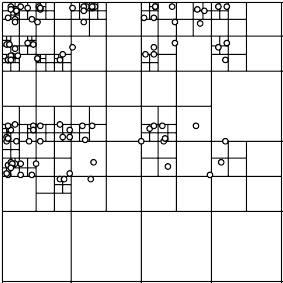
\includegraphics[width=0.3\textwidth]{graphics/test.png}
	\caption{An example QuadTree}
	\label{quadtree_img}
	\vspace{-90pt}
\end{wrapfigure}

The QuadTree is a data structure that is used for storing two-dimensional information in a functional way \cite{Finkel1974}. It is defined as:
\begin{minted}{haskell}
data Quadrant t = Leaf t | Node (Quadrant t) 
	(Quadrant t) (Quadrant t) (Quadrant t)

data QuadTree t = Wrapper (Nat, Nat) (Quadrant t)
\end{minted}

A QuadTree consists of the size (width  ×  height) of the QuadTree, and the root quadrant. A quadrant is either a leaf (in which case all the values inside the region of the quadrant are the same), or four subquadrants. The four subquadrants are then called A (top left), B (top right), C (bottom left), and D (bottom right). Notice that in Figure \ref{quadtree_img}, space is consistently split into four quadrants.

There are five functions that can be used to interact with QuadTrees:
\begin{minted}{haskell}
-- Create a new QuadTree with the specified size
makeTree :: (Nat, Nat) -> t -> QuadTree t
-- Get a lens to the specified location
atLocation :: (Nat, Nat) -> Lens (QuadTree t) t
-- Get the value at the specified location
getLocation :: (Nat, Nat) -> QuadTree t -> t
-- Set the value at the specified location
setLocation :: (Nat, Nat) -> t -> QuadTree t -> QuadTree t
-- Map the value at the specified location
mapLocation :: (Nat, Nat) -> (t -> t) -> QuadTree t -> QuadTree t
\end{minted}

\section{Implementation} \label{implementation}
This section describes how the QuadTree library was implemented in Agda, and what challenges had to be overcome to do so. All the code for this project is available in the public domain. Each directory has a README.md which explains the purpose of all files and folders inside of the directory.
The code is available at: \textcolor{blue}{\href{https://github.com/JonathanBrouwer/research-project}{https://github.com/JonathanBrouwer/research-project}}. 

\subsection{Implementing QuadTree}
The QuadTree library is implemented by composing lenses. The lens that is finally produced is the atLocation lens, which takes a location and a QuadTree, and returns a lens to that location in the QuadTree.
\begin{minted}{agda}
atLocation : (Nat x Nat) -> Lens (QuadTree t) t
\end{minted}
 \verb|atLocation| is implemented by composing \verb|wrappedTree| (which is a lens from a QuadTree to its root quadrant) and  \verb|go|.   The \verb|go| function takes a location and a maximum depth, and returns a lens from a quadrant to the specified location. In its implementation, if the maximum depth is zero, it calls  \verb|lensLeaf|. Otherwise, it composes  \verb|lensA/B/C/D| with a recursive call to itself, that does the rest of the lookup. For example, \verb|go (0 , 0) 5 = lensA ∘ go (0 , 0) 4|.
\begin{minted}{agda}
lensWrappedTree : Lens (QuadTree t) (Quadrant t)
go : (Nat x Nat) -> (depth : Nat) -> Lens (Quadrant t) t
\end{minted}
 \verb|lensLeaf| is a lens from a leaf quadrant to the value stored there. This function has as a precondition that the quadrant has a depth of 0 (a leaf).  \verb|lensA/B/C/D| is a lens from a quadrant to the A/B/C/D sub-quadrant. This function returns a lens from a quadrant with a certain maximum depth to a quadrant with a maximum depth that is one lower. 
\begin{minted}{agda}
lensLeaf : Lens (Quadrant t) t
lensA : Lens (Quadrant t) (Quadrant t)
\end{minted}
 \verb|get/set/mapLocation| can then be defined using the  \verb|atLocation| lens, by composing them with the lens functions. They are shortcut functions so users of the library do not have to interact with lenses directly.
\begin{minted}{agda}
getLocation : (Nat x Nat) -> QuadTree t -> t
getLocation = view ∘ atLocation
setLocation : (Nat x Nat) -> t -> QuadTree t -> QuadTree t
setLocation = set ∘ atLocation
mapLocation : (Nat x Nat) -> (t -> t) -> QuadTree t -> t
mapLocation = over ∘ atLocation
\end{minted}
Finally,  \verb|makeTree| makes a new QuadTree with the same value everywhere, simply by calling the QuadTree constructor
\begin{minted}{agda}
makeTree : (size : Nat × Nat) -> (v : t) -> QuadTree t
\end{minted}

Additionally, QuadTree implements Functor and Foldable. The implementation of functor in the original library breaks one of the QuadTree invariants, so the implementation given in this paper was changed slightly in this implementation to not break this invariant.

\label{total-functions}
\subsection{Issues when converting Haskell to Agda}
A number of issues arise when converting Haskell to Agda, because Agda is a total language and Haskell is not. Being a total language means that every function must terminate and return a value without any run-time errors.

\subsubsection{Termination}
The first issue is encountered when a function in the library is actually non-terminating. This would have to be solved by changing the function, or adding preconditions, such that the function does always terminate. Luckily, all the functions in the QuadTree library do always terminate, so this was not a problem for this paper.

Additionally, the totality of Agda can also be encountered when Agda is not able to automatically prove that a function terminates, even though it does. This did actually occur during the implementation of the QuadTree library in Agda. It was initially solved by adding the \verb|{-# TERMINATING #-}| pragma (which instructs the compiler that this function is terminating) in front of the function, together with an explanation for why the function is definitely terminating. Later on this was solved by expressing the function differently.

\subsubsection{Error}
Finally, while Haskell has some escape latches such as \verb|error|, Agda does not. For example, the \verb|get/set/mapLocation| functions call \verb|error| when the provided location is outside of the QuadTree. This can be solved by adding a precondition to the function, which states that the location must be inside the QuadTree. 

This approach is different from the technique presented in \cite[p. 16]{BREITNER2021}. The technique presented there is making sure that the \verb|error| function may only be used with non-empty types, thus ensuring that the language stays sound. The technique was chosen because it allows for simpler automatic translation from Haskell. Since the translation in this paper is fully manual anyways, this does not add any value. The technique does come with the downside that the function can still be called with an incorrect input in Agda, resulting in an error at runtime rather than compile-time. Adding a precondition to the function prevents this, therefore this has been chosen.

\subsection{Necessary modifications of Agda2hs}
In order to make a working implementation, Agda2hs needed some changes.
\begin{itemize}
    \item Add support for type synonyms (Fixed in \textcolor{blue}{\href{https://github.com/agda/agda2hs/pull/56/}{PR \#56}})
    \item Insert parentheses where required in infix applications (Fixed in  \textcolor{blue}{\href{https://github.com/agda/agda2hs/pull/57/}{PR \#57}})
    \item Support for constructors with implicit arguments (Fixed in  \textcolor{blue}{\href{https://github.com/agda/agda2hs/pull/60/}{PR \#60}})
    \item Instance arguments fail to compile (Fixed in  \textcolor{blue}{\href{https://github.com/agda/agda2hs/pull/66/}{PR \#66}})
    \item Pattern matching on natural numbers does not compile correctly. (Fixed in custom version)
\end{itemize}
The first 4 problems have been solved by the Agda2hs contributors in the official Agda2hs version. The last has not been fixed in the official version, but has been fixed in a custom version which is available at \textcolor{blue}{\href{https://github.com/JonathanBrouwer/agda2hs}{https://github.com/JonathanBrouwer/agda2hs}}. Since this makes some breaking changes to Agda2hs, this has not been submitted as a PR.
\section{Proving Techniques}

The properties that have been proven can be divided into three types: Preconditions, Invariants and Post-conditions \cite{meyer_1992}. Preconditions are properties that must be true before a function is called, post-conditions must be true after a function is called, and invariants are properties that must be true for all values of a certain type. In this section it will be shown that these three types of properties each have their own way to be proven in Agda.

\subsection{Finding properties to prove}\label{finding_props_to_prove}
\cite{BREITNER2021} presents multiple techniques to find properties to prove from Haskell code. A few of those techniques have been selected that were deemed useful for this paper:
\begin{enumerate}
	\item Define an invariant property when there are types whose correctness depend on invariants
		\cite[p. 7]{BREITNER2021}
	\item Define a post-condition property by deriving a definition directly from the test suite
		\cite[p. 9]{BREITNER2021}
	\item Define a precondition when there is a risk of numeric overflow, or switch to using unbounded integers instead. 
		\cite[p. 9]{BREITNER2021}
	\item Define a post-condition when there are type classes which come with laws that all instances of the type class should satisfy
		\cite[p. 10]{BREITNER2021}
\end{enumerate}
Instead of defining a precondition when there is a risk of numeric overflow as described in technique 3, we switch to using unbounded integers in this papers' implementation of the QuadTree library. This is the same decision that \cite{BREITNER2021} made. Furthermore, the test suite of the QuadTree library consists only of tests that test the type class laws, so no additional properties could be derived from technique 2. Finally, one technique that was not mentioned in \cite{BREITNER2021} was used:
\begin{enumerate}
	\setcounter{enumi}{4}
	\item Define a precondition if it is required to make the function total, as was described in section \ref{total-functions}
\end{enumerate}


\subsection{Properties to prove}\label{props_to_prove}
Using technique 1, 4, and 5, the following properties of the QuadTree library were derived: \linebreak 
\textbf{Invariants of a QuadTree:}
\begin{itemize}
    \item Depth invariant: The depth of a QuadTree must be less than or equal to $\left \lceil{log_{2}( max(width, height))}\right \rceil$. This is to ensure that there is exactly one value at each location. (Technique 1)
    \item Compression invariant: No node can have four leaves that are identical. These need to be fused into a single leaf quadrant. This is needed to keep the QuadTree fast and space efficient. (Technique 1)
\end{itemize} 
\textbf{Preconditions of a QuadTree:}
\begin{itemize}
    \item When calling \verb|atLocation|, \verb|getLocation|, \verb|setLocation| or \verb|mapLocation|, the location must be inside of the QuadTree. (Technique 5)
    \item When calling \verb|lensLeaf|, the quadrant needs to have a depth of zero (i.e.  it must be a leaf) (Technique 5)
    \item When calling \verb|lensA/B/C/D|, the quadrant needs to have a depth that is greater than zero (i.e.  it must not be a leaf) (Technique 5)
\end{itemize} 
\textbf{Post-conditions of a QuadTree:}
\begin{itemize}
    \item The lenses returned by all the lens functions satisfy the lens laws: \cite{lens} (Technique 4)
        \begin{itemize}
            \item \verb|view l (set l v s) = v| (Setting and then getting returns the value)
            \item \verb|set l (view l s) s = s| (Setting the value to what it already was doesn't change anything)
            \item \verb|set l v2 (set l v1 s) = set l v2 s| (Setting a value twice is the same as setting it once to the second value)
        \end{itemize}
    \item The functor implementations for Quadrant and QuadTree satisfy the functor laws (Technique 4)
        \begin{itemize}
            \item \verb|fmap id = id| (Identity law)
            \item \verb|fmap (f . g) == fmap f . fmap g| (Composition law)
        \end{itemize}
    \item The foldable implementation returns an output of the correct length (Technique 4)
        \begin{itemize}
            \item \verb|length quadtreeFoldable vqt = width * height|
        \end{itemize}
    \item The foldable implementation satisfies the foldable-functor law (Technique 4)
        \begin{itemize}
            \item \verb|foldMap f = fold . fmap f|
        \end{itemize}
\end{itemize}

\subsection{Techniques to prove invariants} \label{prove_invariants}
Invariants are proven by creating a new datatype with one constructor, which takes the original datatype and a proof for all the invariants. As a simple example, this datatype represents a natural number with the invariant that it is greater than 5.
\begin{minted}{agda}
data GreaterThanFive : Set where
  CGreaterThanFive : (n : Nat) -> { .( IsTrue (n > 5) ) } -> GreaterThanFive
\end{minted}
The proof is marked as implicit \{\} so that it is removed when compiled to Haskell, and it is marked as as irrelevant .() so that will not interfere when proving post-conditions later. An irrelevant value means that the actual value of the proof does not matter, only its existence does.

Using this technique, the datatype for a compressed quadrant with a certain maximum depth is: 
\begin{minted}{agda}
data VQuadrant (t : Set) {depth : Nat} : Set where
  CVQuadrant : (qd : Quadrant t) 
            -> {.(IsTrue (depth qd <= depth && isCompressed qd))} 
            -> VQuadrant t {depth}
\end{minted}
The datatype for a valid QuadTree is defined very similarly. Agda2hs flawlessly compiles this to the following Haskell code, where the proof is erased:
\begin{minted}{haskell}
data VQuadrant t = CVQuadrant (Quadrant t)
\end{minted}

The advantage of making a new wrapper datatype over adding the proofs to the original datatype is that if the original datatype has multiple constructors, functions that use the proof do not need to be split into multiple cases (one for each constructor). The disadvantage is that this additional wrapper type is visible when compiled to Haskell. To avoid this, it is possible to create an additional function for all public functions. This function then takes the invariance proof as a precondition, and calls the original function with the wrapper type. 

\subsection{Techniques to prove preconditions}
In this section, two techniques to prove preconditions are presented.

\subsubsection{Using an implicit argument} \label{using_implicit}
When using the implicit argument technique, preconditions are proven by adding the proofs as implicit arguments to the function.
As a simple example, this function takes a natural number that must be greater than 5.
\begin{minted}{agda}
takesGtFive : (n : Nat) -> { .( IsTrue (n > 5) ) } -> ?
\end{minted}
As with invariants, the proof is marked as implicit and irrelevant. 

Using this technique, a precondition can be used to ensure that the location given to the getLocation function must be inside the QuadTree:
\begin{minted}{agda}
-- Function that checks if a location is inside a given QuadTree
isInsideQuadTree : (Nat × Nat) -> QuadTree t -> Bool
isInsideQuadTree (x , y) (Wrapper (w , h) _) = x < w && y < h

getLocation : (loc : Nat × Nat) -> (qt : QuadTree t) 
    -> {.( IsTrue (isInsideQuadTree loc qt) )} -> t
\end{minted}
After being compiled with Agda2hs, the precondition is removed from the function, just like with invariants.
\begin{minted}{haskell}
getLocation :: (Nat, Nat) -> QuadTree t -> t
\end{minted}

\subsubsection{Using a datatype with invariants}
Another technique to prove preconditions is by passing in a datatype with an invariant, as was used in section \ref{prove_invariants}. The simple example from \ref{using_implicit} would then be written like this, using the type defined in section \ref{prove_invariants}:
\begin{minted}{agda}
takesGtFive : (n : GreaterThanFive) -> ?
\end{minted}

For the QuadTree verification, this technique was used to encode the maximum depth properties of the lens functions, using the same datatype that was defined for the invariants.
\begin{minted}{agda}
lensLeaf : Lens (VQuadrant t {0}) t
lensA : {dep : Nat} 
    -> Lens (VQuadrant t {S dep}) (VQuadrant t {dep})
\end{minted}

\subsubsection{Comparison}
The advantages of using implicit arguments is that it is not necessary to define a separate datatype, and that the precondition can be dependent on more than one parameter of the function. On the other hand, the advantages of using a datatype with an invariant is that the defined function are cleaner and more compact. It is then also possible to use the type as a parameter for another type, like it is used in \verb|lensLeaf| and \verb|lensA|. It also allows for cleaner reuse of the property, as it does not need to be repeated each time it is used.

\subsection{Techniques to prove post-conditions}
Post-conditions are proven as separate functions. As a simple example, this is a proof that this function returns a number greater than 5.
\begin{minted}{agda}
gt5 : Bool -> Nat
gt5 _ = 42

gt5-is-gt5 : (b : Bool) -> IsTrue (gt5 b > 5)
gt5-is-gt5 b = IsTrue.itsTrue
\end{minted}

For the QuadTree verification, this technique was used to verify the lens laws of all the lenses defined in the implementation. For example, this is the proof that the ViewSet law holds for \verb|lensLeaf|.
\begin{minted}{agda}
ValidLens-Leaf-ViewSet : 
    -> (v : t) (s : VQuadrant t {0}) 
    -> view (lensLeaf {t}) (set (lensLeaf {t}) v s) ≡ v
ValidLens-Leaf-ViewSet v (CVQuadrant (Leaf x)) = refl
\end{minted}

When proving preconditions and invariants, these properties have to be marked as irrelevant. This is to ensure that when proving that two function calls are equal, one does not need to show that the proofs of the preconditions and invariants are equal, since the actual value of the proofs is irrelevant.

\subsection{Results} \label{results}
All of the properties mentioned in section \ref{props_to_prove} have been successfully proven. Most of these proofs have not been shown in the paper, since they are available in the source code. The amount of lines of code that this took is shown in figure \ref{division}.  This counts all non-empty lines. The verification took about 3 times more lines of code than the implementation. While this comparison is an indication, this should not be taken to mean that the verification took 3 times as much effort, as the information density of the implementation and proofs is different.

In reality, the implementation took approximately one full-time week, while the verification took approximately five full-time weeks. This too should not be taken to mean the verification took 5 times as much effort, as this number may be biased by the fact that the implementation was just translation from Haskell.

During the verification phase, one bug was found in this papers implementation of QuadTree that was accidentally introduced during the translation to Agda. This was not caught by the tests, though this may be because the tests on the foldable implementation are very limited.

Whether this time is worth the time spent, depends on the situation. For example, in a situation where even one small error could bring down an airplane, this is clearly worth it. However, in many common situations, this verification may not be worth it.

\begin{figure}[H]
	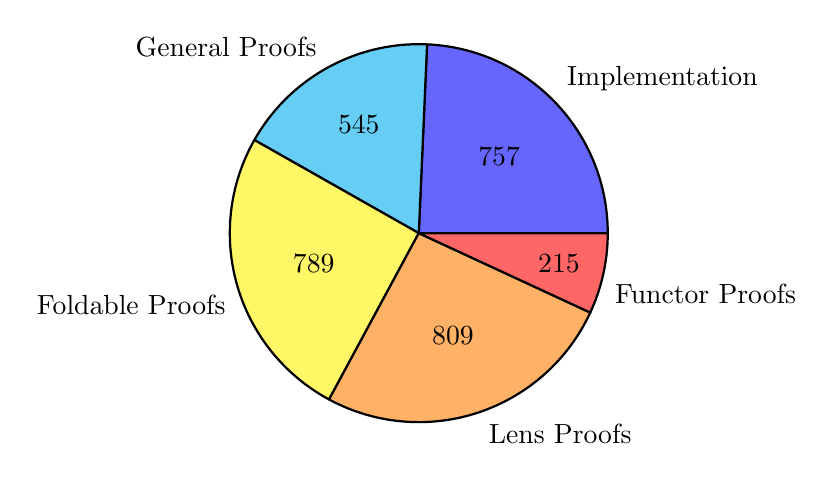
\begin{tikzpicture}[scale=0.8]
		\pie[sum=auto]
		{757/Implementation,
			545/General Proofs,
			789/Foldable Proofs,
			809/Lens Proofs,
			215/Functor Proofs}
	\end{tikzpicture}
	\caption{Division of lines of code}
	\label{division}
\end{figure}
\section{Responsible Research}
In this paper the QuadTree library is implemented and verified, and the techniques (method) used to do so are presented. These techniques are written with the goal that a reader who is trying to implement and verify their own library, can do so using these techniques, and reproduce the results. When there are doubts on how these techniques are actually applied, the code for this project is released on GitHub, so anyone who wants to verify that the techniques really work can see how they were applied in this project. It is also important that other research which aims to improve on the ideas presented in this paper, can do so. This is why the code is released to the public domain, so other researchers can use it and improve on it in their research.
\section{Discussion}
\subsection{Reducing the time required for verification}
In this section, some techniques used to speed up the verification process are presented. First of all, these are some techniques to reduce the time required for verification:
\begin{itemize}
    \item Postulate theorems about libraries. For example, proving that the following 3 statements about lenses are true, turned out to be difficult enough that it was not worth doing. Intuitively these are clearly true, but proving this in Agda takes a lot of time which depending on the situation may not be worth it. 
    \begin{minted}{agda}
    view (l1 ∘ l2) ≡ view l2 ∘ view l1
    set (l1 ∘ l2) ≡ over l1 (set l2 t) v
    over l ≡ set l (view l v) v
    \end{minted}
    \item Use Agda automatic proof search. Automatic proof search often doesn't find a solution, but sometimes it does, and trying it does not cost anything.
    \item First prove invariants and preconditions, then prove postconditions. Invariants and preconditions change the signature of the function, so when any of them are changed, the proofs for postconditions have to be updated.
\end{itemize}

Additionally, there are some long-term recommendations I would like to make to improve the process of verifying code in Agda:
\begin{itemize}
    \item It would be useful to have a better interface to search common proofs which already exist. It is difficult for a novice Agda programmer to find and use the proofs that are already in the standard library. For example, associativity and commutativity of addition and multiplication do not have "associativity" or "commutativity" in their name, though even if they did, there is no easy way to search the names of proofs.
    \item Improvements to automatic proof search would be useful. The automatic proof search often doesn't find a solution, even if the proof is relatively simple. For example, it cannot find a relatively simple proof such as (a + b) + c ≡ a + (b + c). This is because the proof requires cong and case splitting, which the automatic proof search is not allowed to do by default. Giving it the options `-c cong` makes it find the proof quickly, but this is bothersome.
\end{itemize}
\section{Conclusions and Future Work}
In this paper, the QuadTree library is implemented and verified in the subset of Agda that agda2hs supports to determine whether agda2hs can be used to produce a verified implementation of a Haskell library. After some minor modifications to agda2hs, the library has successfully been implemented. Then, the library was verified by verifying invariants by creating a datatype which takes the proof, verifying preconditions by adding the proofs as implicit arguments to the function or by passing in a datatype with an invariant, and postconditions are proven as separate functions.  Then, it is shown that verification can be sped up by postulating theorems about libraries that are used. Using these techniques, all the properties that were attempted to be verified, have been verified. MORE POSITIVE + INCLUDE BIAS OF ALREADY HAVING IMPLEMENTATION

The techniques presented have only been used to verify this library, it is possible that other libraries cannot be verified using these techniques, so more research should be done to obtain general conclusions by trying to use these techniques with other libraries.


\bibliographystyle{unsrt}
\bibliography{bibliography}

\end{document}
